%Results
\section{Descriptive statistics}
Before the experiment, the seeds were weighted in groups of ten, to see if there was a baseline difference between certain genotypes. Table \ref{tab:germination_percentage}, in the previous section, displays the measured weights.
After the completion of the experiment, the outliers were identified, and each plant was attributed a specific weight, following the protocol described in material and methods section. Those weights were used to compute the weighted mean and weighted standard deviation of the fresh and dry weight of the root system and the leaf system, as well as the area of the root system, for each plant. Dotplots representing those descritptive statistics as well as the data point are presented in figure \ref{fig:dotplot_all_variables}. The numerical values of these results are presented in table \ref{tab:summary_table_all_variables}, in appendix \ref{appendix:mean_std_table}.\\

Even though no clear conclusions can be made from these figures, we can see large variation of mean values between genotypes. Also, for some genotypes, the difference between tanks seem significant (e.g. genotype 15) while it's clearly not the case for some other (e.g. genotype 7). This implies that the tank and genotypes effects are significant. Overall the values of dry weights seem to have less variations than the fresh weights.

\begin{figure}
\centering
	\begin{subfigure}[t]{\textwidth}
		\centering
		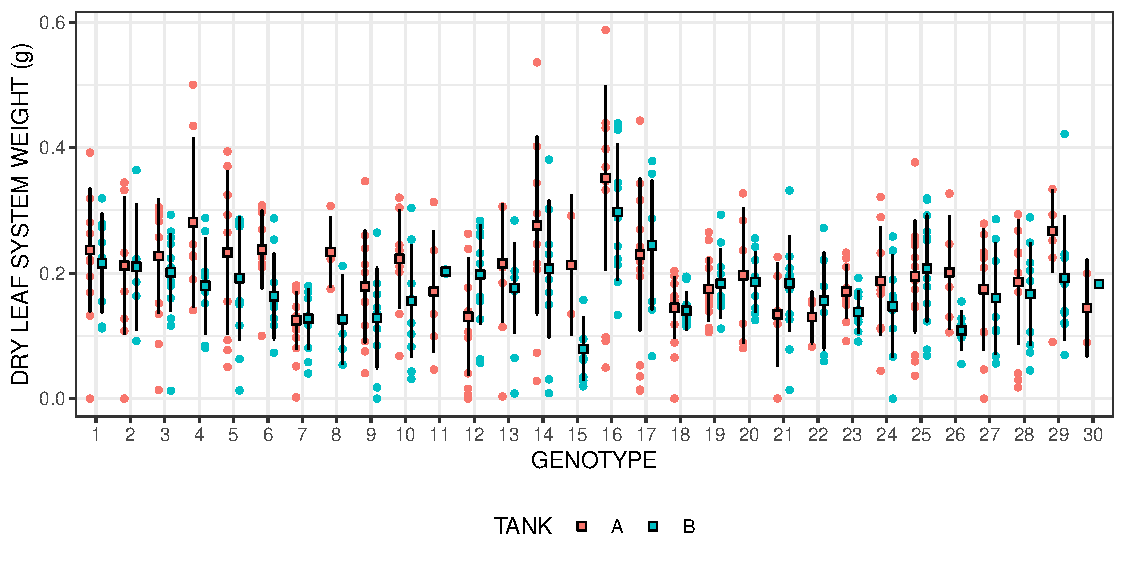
\includegraphics[width = \textwidth]{../../Figures/DRY_LS_summary_plot.pdf}
		\caption{Dry leaf weight ($DRY\_LS$)}
	\end{subfigure}

	\begin{subfigure}[t]{\textwidth}
		\centering
		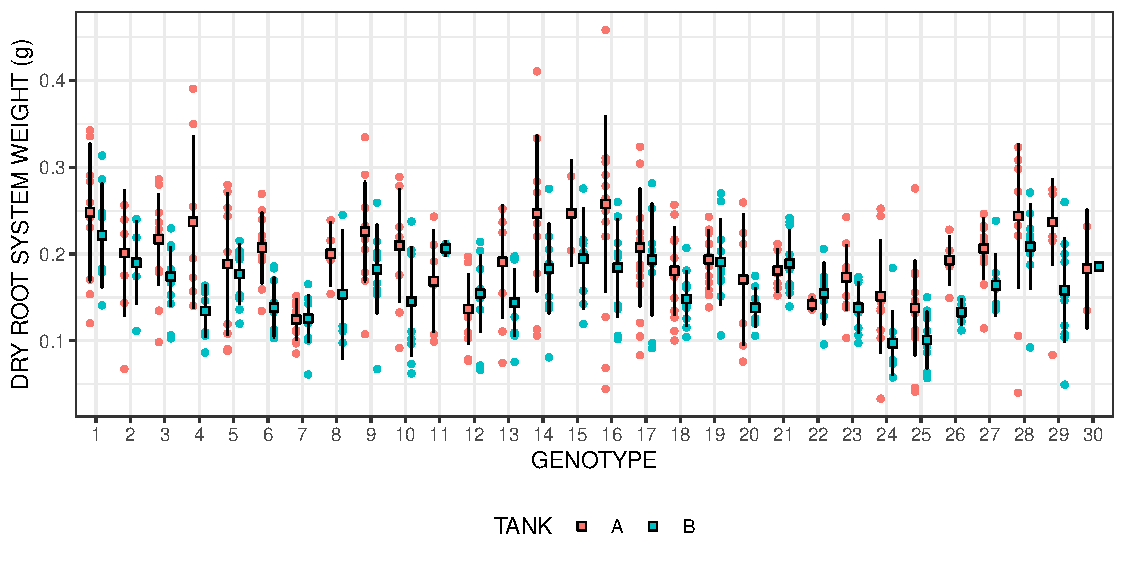
\includegraphics[width = \textwidth]{../../Figures/DRY_RS_summary_plot.pdf}
		\caption{Dry root weight ($DRY\_RS$)}
	\end{subfigure}
	\caption[Dotplot of the mean weight and associated standard deviation]{Dotplot displaying mean weight (\protect\emptysquare) and associated standard deviation (\protect\blackline), grouped by tanks for each variable.}
\end{figure}
\begin{figure}\ContinuedFloat
	\begin{subfigure}[t]{\textwidth}
		\centering
		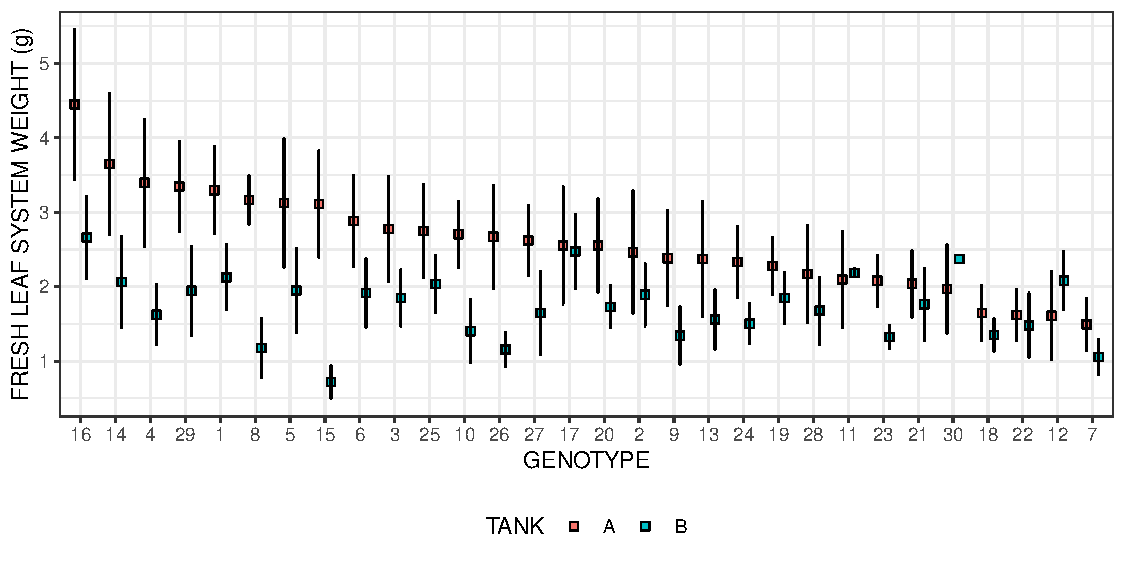
\includegraphics[width = \textwidth]{../../Figures/FRESH_LS_summary_plot.pdf}
		\caption{Fresh leaf weight ($FRESH\_LS$)}
	\end{subfigure}

	\begin{subfigure}[t]{\textwidth}
		\centering
		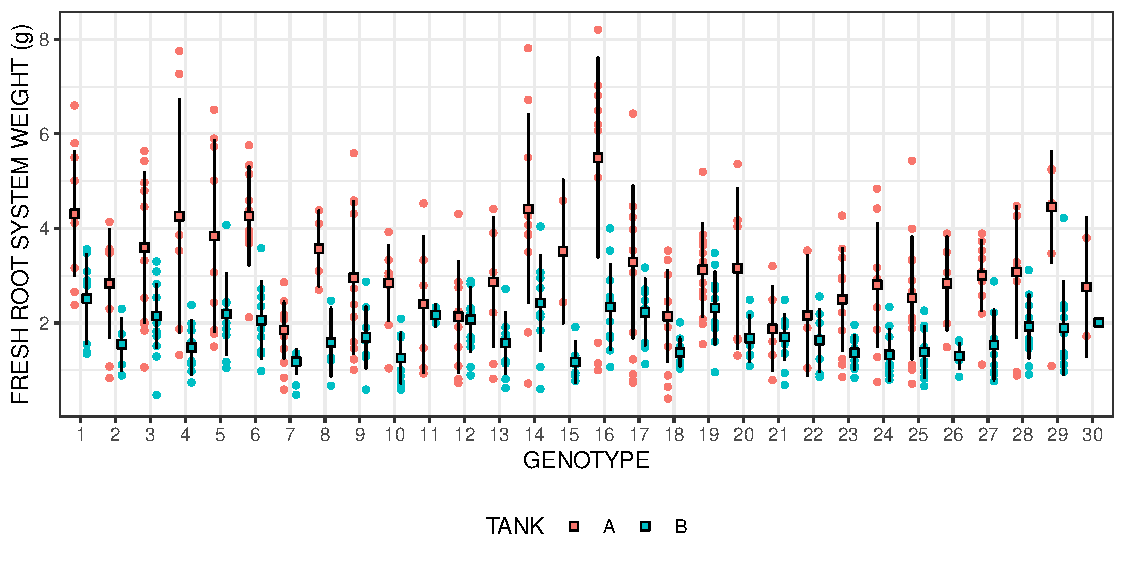
\includegraphics[width = \textwidth]{../../Figures/FRESH_RS_summary_plot.pdf}
		\caption{Fresh root weight ($FRESH\_RS$)}
	\end{subfigure}
	\caption[Dotplot of the mean weight and associated standard deviation]{Dotplot displaying mean weight (\protect\emptysquare) and associated standard deviation (\protect\blackline), grouped by tanks for each variable.}
	\label{fig:dotplot_all_variables}
\end{figure}

\section{SpATS analysis}
The SpATS model was fitted using the four weight variables. The effective dimension of the spatial components, the residuals and the genotype components are presented in table \ref{tab:spats_dimensions}. We see clearly that ...

% Table generated by Excel2LaTeX from sheet 'Sheet2'
\begin{table}[htbp]
  \centering
  \caption[Effective dimensions of the SpATS model]{Model dimensions and effective dimensions (and percentage of the total of 
  the spatial components) of each spatial components for all variables. $ED_{\epsilon}$ represents the effective dimensions for 
  the residuals; $ED_{g}$, is the effective dimensions for the genotype and $H_{g}^2$ is the heritability. Here $\mathbf{v}$ 
  represents the columns, i.e. the position on the strip; and $\mathbf{u}$ represents the rows, i.e. the strip itself.}
    \begin{tabular}{lrrrrr}
    \toprule
    Model components & \multicolumn{1}{c}{Model} & \multicolumn{1}{l}{FRESH\_LS} & \multicolumn{1}{l}{FRESH\_RS} & \multicolumn{1}{l}{DRY\_LS} & \multicolumn{1}{l}{DRY\_RS} \\
    \midrule
    $f_{v}(\mathbf{v})$ & 6     & 0 (0,00\%) & 0 (0,00\%) & 0 (0,00\%) & 0 (0,00\%) \\
    $f_{u}(\mathbf{u})$ & 100   & 0,8 (8,73\%) & 2,26 (14,10\%) & 1,02 (17,26\%) & 1,8 (17,26\%) \\
    $\boldsymbol{u} \odot h_{v}(\boldsymbol{v})$ & 6     & 1,84 (19,95\%) & 2,63 (16,40\%) & 1,47 (24,77\%) & 2,54 (24,77\%) \\
    $\boldsymbol{v} \odot h_{u}(\boldsymbol{u})$ & 100   & 0,24 (2,56\%) & 0 (0,00\%) & 1,09 (18,36\%) & 0,49 (18,36\%) \\
    $f_{u, v}(\boldsymbol{u}, \boldsymbol{v})$ & 150   & 6,33 (68,76\%) & 11,16 (69,50\%) & 2,35 (39,62\%) & 0,08 (39,62\%) \\
    \midrule
    $ED_{\epsilon}$ &       & 466.6 & 459,3 & 470,2 & 470,1 \\
    \midrule
    $ED_{g}$  & 30    & 21,02 & 22,58 & 21,38 & 22,98 \\
    $H_{g}^2$ &       & 0,72  & 0,78  & 0,74  & 0,79 \\
    \bottomrule
    \end{tabular}%
  \label{tab:spats_dimensions}%
\end{table}%

Figure \ref{}

\begin{sidewaysfigure}
	\begin{subfigure}[t]{0.3 \textheight}
		\centering
		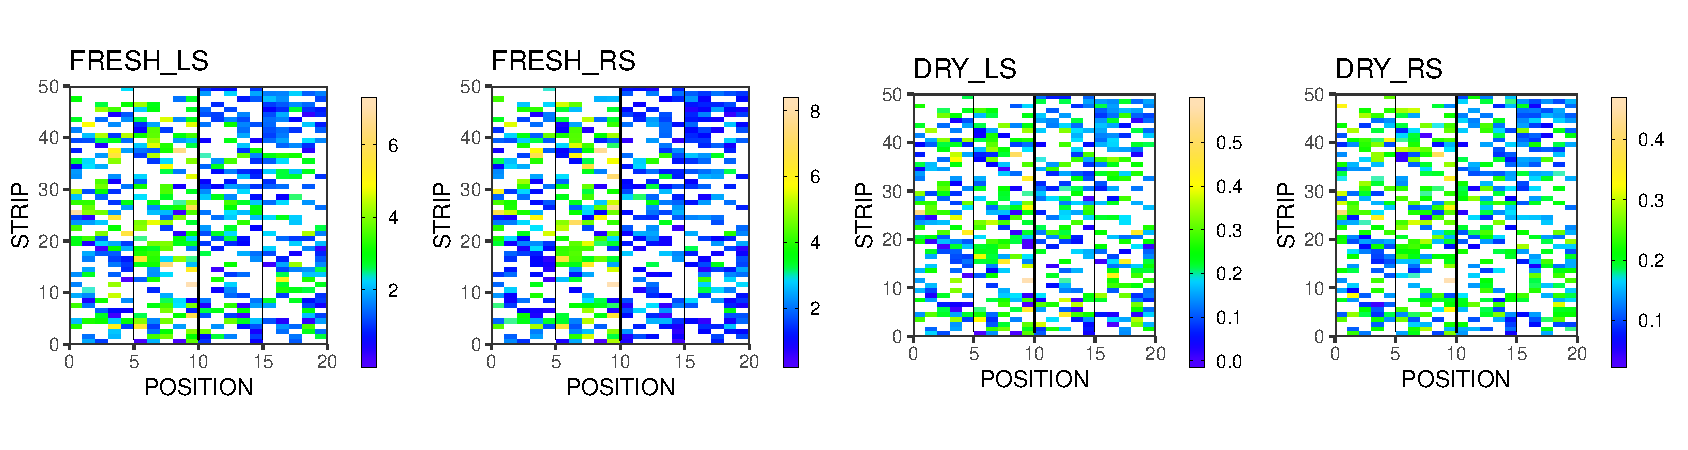
\includegraphics[width = \textwidth]{../../Figures/rawData_plot.pdf}
		\caption{Raw data}
	\end{subfigure}
	
	\begin{subfigure}[t]{0.3 \textheight}
		\centering
		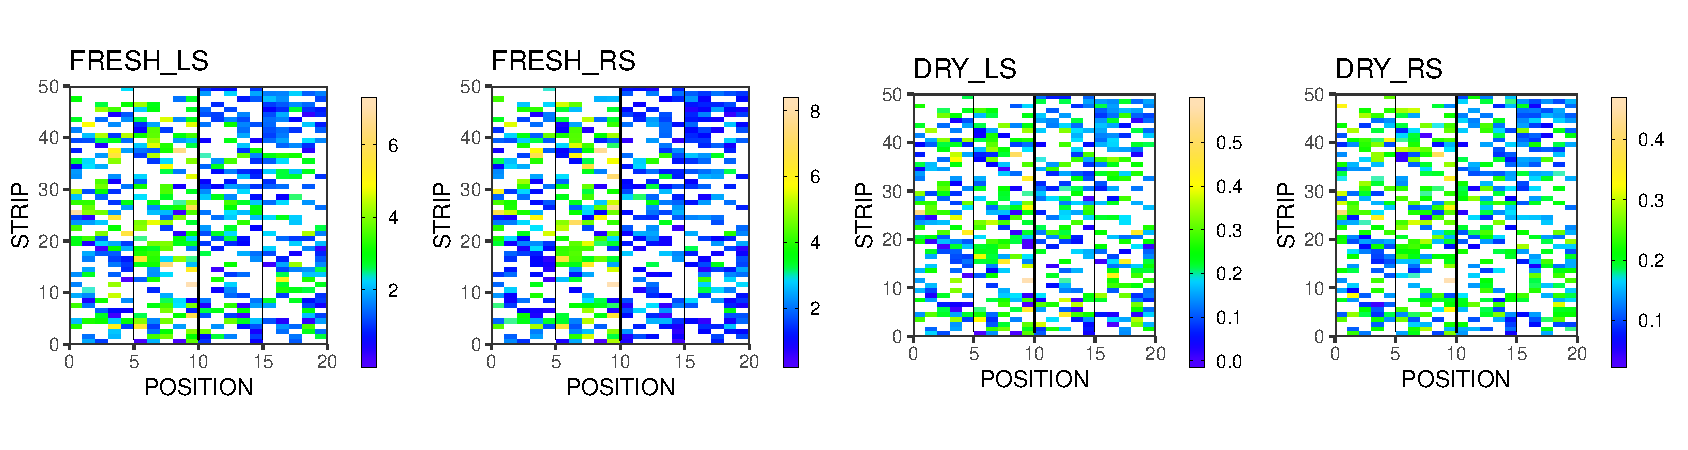
\includegraphics[width = \textwidth]{../../Figures/rawData_plot.pdf}
		\caption{Raw data}
	\end{subfigure}
	
	\begin{subfigure}[t]{0.3 \textheight}
		\centering
		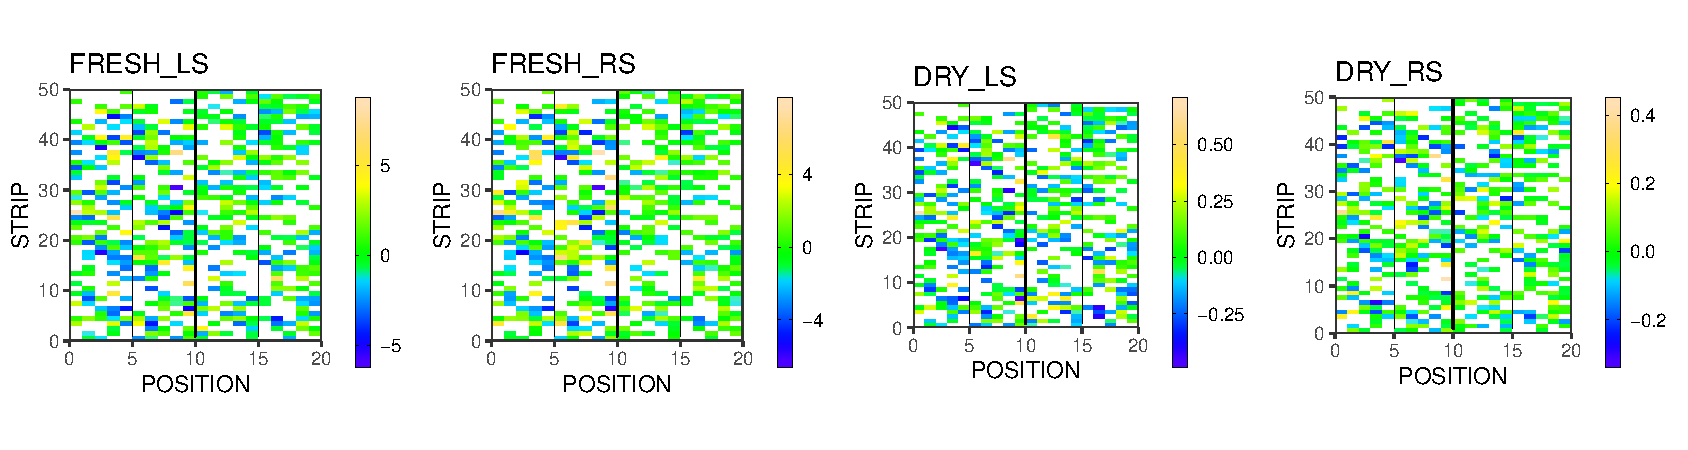
\includegraphics[width = \textwidth]{../../Figures/residuals_plot.pdf}
		\caption{Residuals' spatial plot}
	\end{subfigure}
	\caption{Raw data; fitted spatial trend and residuals' plot for each variable.}
\end{sidewaysfigure}

\section{ARxAR model analysis}
\section{Model comparison}
\subsection{Performances}
\subsection{Parametrization}
\subsection{Modelling strategy}
